\chapter{Triangles}\label{ChTriangles}

\begin{acquis}
\begin{itemize}
\item reconnaître des triangles particuliers;
\item construire un triangle quelconque ou particulier à partir d'une figure à main levée et d'un énoncé;
\item trouver l'orthocentre d'un triangle;
\item trouver le centre de gravité d'un triangle;
\item tracer le cercle inscrit dans un triangle;
\item tracer le cercle circonscrit à un triangle.
\end{itemize}
\end{acquis}

\activites
\begin{activite}[Du côté des triangles \ldots]

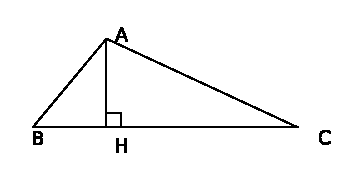
\includegraphics[width=4.8cm]{triangleABCH}

\begin{enumerate}
\item Donne d'autres écritures de l'angle $\widehat{ABC}$ \dotfill

\item Quel angle du triangle $AHC$ possède la plus petite mesure ?  \dotfill

\item Dans le triangle $ABC$, quel est le côté opposé au sommet $B$ ?  \dotfill

\item Dans le triangle $AHC$, quel est le sommet opposé au côté $[HC]$ ?  \dotfill

\item Quel est l'angle droit du triangle $HAB$ ?  \dotfill

\item Quels sont les noms des trois angles du triangle $ACH$ ?  \dotfill

\item Dans cette figure, quels sont les angles aigus, droits et obtus ?  \dotfill

 \dotfill

 \dotfill
\end{enumerate}

\end{activite}

%%%%%%%%%%%%%%%%%%%%%%%%%%%%%%%%%%%%%%%%%%%%%%%%%%%%%%%%%%%%%%%

\begin{activite}[Du côté des triangles particuliers \ldots]

Romuald doit construire un triangle $IJK$ rectangle en $I$, Isabelle un triangle $EFG$ isocèle en $F$ et Eddy un triangle équilatéral $QRS$.

\begin{enumerate}

\item Trace trois figures à main levée pour représenter ces triangles et code-les.

\vspace{4cm}
\item Dans le triangle $IJK$, quel nom donne-t-on au côté $[JK]$ ? \dotfill

\item Dans le triangle $EFG$, quelle est la base ? Quel est le sommet principal ? Que peut-on dire des côtés $[EF]$ et $[GF]$ ? Que peut-on dire des angles $\widehat{FEG}$ et $\widehat{FGE}$ ?  \dotfill

 \dotfill

\item Que peut-on dire des côtés du triangle $QRS$ ? Et de ses angles ?  \dotfill

\item En observant le codage, indique la nature des triangles ci-dessous :


\includegraphics[width=2.3cm]{triangle_rose} \hfill 
\includegraphics[width=1.8cm]{triangle_vert} \hfill 
\includegraphics[width=2.1cm]{triangle_bleu} \hfill 
\includegraphics[width=1.9cm]{triangle_orange}

\end{enumerate}

\end{activite}

%%%%%%%%%%%%%%%%%%%%%%%%%%%%%%%%%%%%%%%%%%%%%%%%%%%%%%%%%%%%%%%

\begin{activite}[Somme des angles d'un triangle]

\begin{enumerate}
\item Trace deux triangles quelconques de formes différentes et mesure leurs angles à l'aide d'un rapporteur.

\item Trace un triangle particulier (isocèle, rectangle ou équilatéral) puis mesure ses angles à l'aide d'un rapporteur.

\item Pour chacun des trois triangles tracés, additionne les mesures de ses trois angles. Que remarques-tu ?

\item Essaie de tracer un triangle dont la somme des angles vaut $220^\circ°$. Que remarques-tu ?
\end{enumerate}

\end{activite}

%%%%%%%%%%%%%%%%%%%%%%%%%%%%%%%%%%%%%%%%%%%%%%%%%%%%%%%%%%%%%%%

\begin{activite}[Hasardons-nous à construire un triangle]

\begin{enumerate}
\item Choisis trois nombres compris entre 2 et 15. Note-les sur ton cahier. Effectue un croquis d'un triangle dont les trois nombres choisis sont les mesures de ses côtés (en cm).

\item Essaie de le construire en vraie grandeur.

\item Penses-tu qu'il soit possible de construire le triangle représenté par le croquis ci-dessous ? Justifie.

\begin{center} 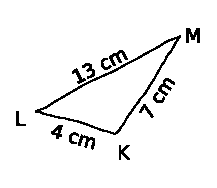
\includegraphics[width=2.9cm]{triangleLMK} \end{center}
\end{enumerate}

\end{activite}

%%%%%%%%%%%%%%%%%%%%%%%%%%%%%%%%%%%%%%%%%%%%%%%%%%%%%%%%%%%%%%%

\begin{activite}[Constructible ou non ?]
Un professeur demande à ses élèves de construire le triangle $ABC$ donné par le croquis ci-contre. Voici les réponses de quatre élèves : \\[1em]
\begin{minipage}[t]{0.46\textwidth}
\begin{itemize}
 \item Kim dit que le triangle $ABC$ est constructible puisque la figure est tracée ;
 \item Jordan dit que, comme $4 < 6 + 11$,  le triangle $ABC$ est constructible ;
 \item Mickaël dit qu'il est d'accord avec Jordan car en plus $6 < 11 + 4$ ;
 \item Imad dit que l'inégalité $11 < 6 + 4$ est fausse et que le triangle $ABC$ n'est donc pas constructible.
 \end{itemize}
\end{minipage} \hfill%
\begin{minipage}[t]{0.36\textwidth}
\hfill \\
\begin{center} 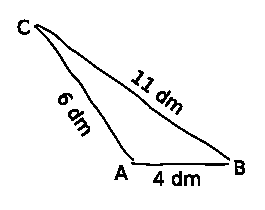
\includegraphics[width=3.8cm]{triangleCAB} \end{center}
\end{minipage} \\

\begin{enumerate}
\item Que penses-tu de chacune des réponses ? Qui a raison ?

\item Au total, combien d'inégalités ont été proposées par ces élèves ? Pour savoir si le triangle $ABC$ est constructible, faut-il vérifier toutes ces inégalités ?
   
\item Effectue un croquis d'un triangle \underline{non} constructible ayant des côtés mesurant 7,5 m, 12 m et une troisième valeur de ton choix, plus grande que les deux autres.
         
\item Effectue un croquis d'un triangle \underline{non} constructible ayant des côtés mesurant 6,5 km, 10 km et une troisième valeur de ton choix, plus petite que les deux autres.
\end{enumerate}

\end{activite}


%%%%%%%%%%%%%%%%%%%%%%%%%%%%%%%%%%%%%%%%%%%%%%%%%%%%%%%%%%%%%%%

\begin{activite}[Une figure à main levée \ldots à l'œil ouvert]

Voici quatre croquis d'un triangle $AKL$ tel que $AK = 5$ cm, $\widehat{LAK} = 47^\circ$ et $\widehat{LKA} = 96^\circ$ :
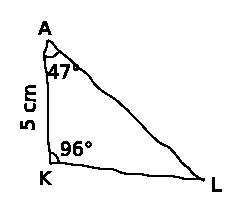
\includegraphics[width=3.3cm]{triangleAKL_1} \hfill 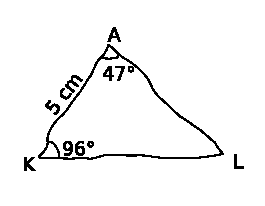
\includegraphics[width=3.4cm]{triangleAKL_2} \hfill 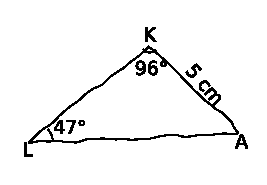
\includegraphics[width=3.8cm]{triangleAKL_3} \hfill 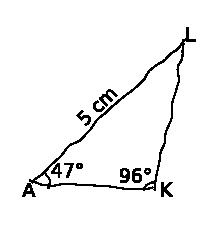
\includegraphics[width=2.7cm]{triangleAKL_4}

\qquad croquis 1 \hfill croquis 2 \hfill croquis 3 \hfill croquis 4 \hfill \\[0.2em]

\begin{enumerate}

\item Quels sont les croquis corrects ?  \dotfill

\item Construis le triangle $AKL$.
\end{enumerate}

\end{activite}


%%%%%%%%%%%%%%%%%%%%%%%%%%%%%%%%%%%%%%%%%%%%%%%%%%%%%%%%%%%%%%%

\begin{activite}[Une figure à main levée \ldots à l'œil ouvert (bis)]

Voici cinq croquis d'un triangle $NPS$ isocèle en $N$ tel que $NS = 4$ cm et $\widehat{SNP} = 75^\circ°$ :

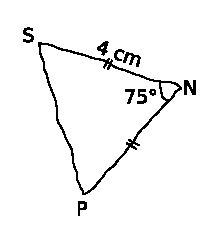
\includegraphics[width=2.6cm]{triangleSNP_1} \hfill 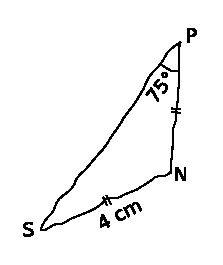
\includegraphics[width=2.4cm]{triangleSNP_2} \hfill 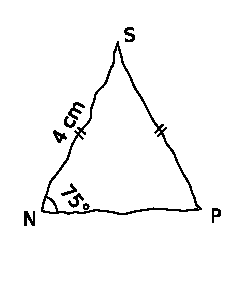
\includegraphics[width=2.9cm]{triangleSNP_3} \hfill 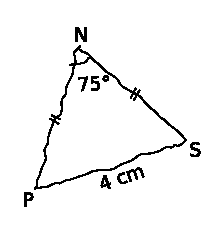
\includegraphics[width=2.7cm]{triangleSNP_4} \hfill 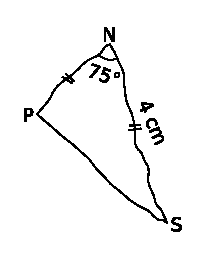
\includegraphics[width=2.5cm]{triangleSNP_5} 

\quad croquis 1 \hfill croquis 2 \hfill croquis 3 \hfill croquis 4 \hfill croquis 5 \\[0.2em]

\begin{enumerate}

\item Quels sont les croquis corrects ? \dotfill

\item En commençant par le segment $[NS]$, construis le triangle $NPS$.
\end{enumerate}

\end{activite}


\cours

%\section{Une section}

% remarque : pour qu'un mot se retrouve dans le lexique : \MotDefinition{asymptote horizontale}{} 
\begin{definition}
Un \MotDefinition{triangle isocèle}{} est un triangle qui a deux côtés égaux;

un \MotDefinition{triangle équilatéral}{} est un triangle qui a trois côtés égaux;

un \MotDefinition{triangle rectangle}{} est un triangle qui a deux côtés perpendiculaires.
\end{definition}

\begin{methode*1}[Construire un triangle]

\begin{exemple*1}
Construis un triangle $KLM$ tel que $KL = 6$ cm ; $LM = 5$ cm et $KM = 4,5$ cm :

On trace une figure à \textbf{main levée} :
\begin{center} 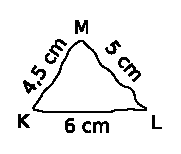
\includegraphics[width=2.3cm]{triangleKML} \end{center}

\begin{tabularx}{\textwidth}{X|X|X}
 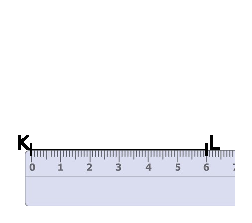
\includegraphics[width=3.1cm]{regleKL} &  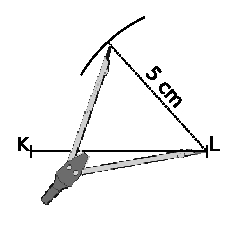
\includegraphics[width=3.1cm]{compasKL} & 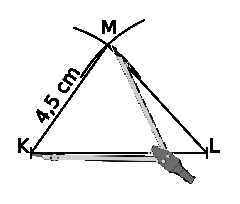
\includegraphics[width=3.1cm]{compasKML} \\ 
 On trace un segment $[KL]$ de longueur 6 cm. & Le point $M$ est à 5 cm du point $L$ : il appartient au cercle de centre $L$ et de rayon 5 cm. & Le point $M$ est à 4,5 cm du point $K$ : il appartient au cercle de centre $K$ et de rayon 4,5 cm. \\
\end{tabularx} \\

\end{exemple*1}

\exercice 
Construis un triangle $VOL$ tel que :

$VO = 4$ cm ; $OL = 6,3$ cm et $LV = 3,8$ cm.

\vspace{2cm}
%\correction

\exercice 
Construis un triangle \textbf{équilatéral} $EAU$ de 45 mm de côté.

\vspace{2cm}
%\correction

\exercice 
Construis le triangle $UNO$ \textbf{isocèle} en $U$ avec :

$UN = 8$ cm et $NO = 3,6$ cm.
%\correction
 
\end{methode*1}

%%%%%%%%%%%%%%%%%%%%%%%%%%%%%%%%%%%%%%%%%%%%%%%%%%

\begin{methode*1}[Construire un triangle rectangle]

\begin{exemple*1}
Construis un triangle $KHI$ rectangle en $K$ tel que $KI = 5$ cm et $HI = 7$ cm : \\[1em]
\begin{tabularx}{\textwidth}{X|X|X|X}
 On trace un segment $[KI]$ de longueur 5 cm (dessins suivants agrandis). & On trace la droite perpendiculaire en $K$ à $(KI)$ et on code l'angle droit. & On trace un arc de cercle de centre $I$ et de rayon 7 cm coupant la perpendiculaire en $H$. & On trace le segment $[HI]$.\\
 
\includegraphics[width=2.2cm]{regle5} & 
\includegraphics[width=1.8cm]{equerreKI} & 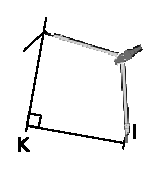
\includegraphics[width=2cm]{compasKI} & 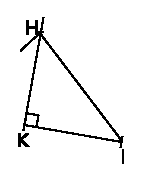
\includegraphics[width=1.8cm]{triangleHKI} \\ 
\end{tabularx} \\

\end{exemple*1}

\exercice 
Construis un triangle $MDR$ rectangle en $D$ tel que :

$MD = 4,2$ cm et $DR = 7,1$ cm. 
\vspace{4cm}
%\correction
 
\exercice
Construis un triangle $ILE$ rectangle en $E$ tel que :

$EL = 6,4$ cm et $LI = 9,3$ cm.
\vspace{2cm}
%\correction
 
\end{methode*1}

%%%%%%%%%%%%%%%%%%%%%%%%%%%%%%%%%%%%%%%%%%%%%%%%%%

\begin{methode*1}[Construire un triangle connaissant un angle et les longueurs \\ de ses côtés adjacents]

 \begin{exemple*1}
Construis un triangle $BAS$ tel que :

$AB = 10,4$ cm ; $BS = 8$ cm et $\widehat{ABS} = 99^\circ$ : \\[1em]
\begin{tabularx}{\textwidth}{X|X|X}
 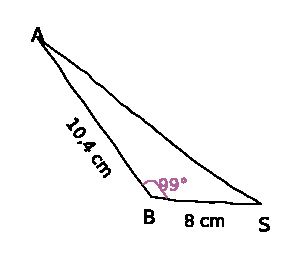
\includegraphics[width=3.3cm]{triangleABS} &  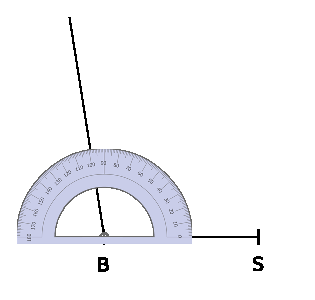
\includegraphics[width=3.5cm]{rapporteurBS} & 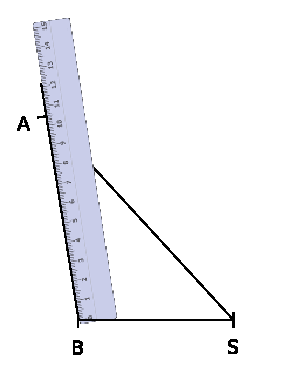
\includegraphics[width=3.6cm]{regleABS} \\ 
 On effectue une figure à main levée en respectant la nature des angles (aigu ou obtus). & On construit un segment $[SB]$ de 8 cm de longueur. On trace un angle mesurant $99^\circ$ de sommet $B$ et de côté $[BS)$. & On place le point $A$ sur le côté de l'angle à 10,4 cm du point $B$. \\
\end{tabularx} \\

\end{exemple*1}

\exercice
Construis un triangle $LET$ tel que :

$\widehat{ETL} = 55^\circ$ ; $ET = 5$ cm et $TL = 4,3$ cm.
\vspace{4cm}
%\correction

\exercice
Construis un triangle $SEL$ tel que :

$SL = 6,4$ cm ; $\widehat{SLE}= 124^\circ$ et $LE = 7,9$ cm.
\vspace{2cm}
%\correction
 
\end{methode*1}


%%%%%%%%%%%%%%%%%%%%%%%%%%%%%%%%%%%%%%%%%%%%%%%%%%

\begin{methode*1}[Construire un triangle connaissant deux angles et la longueur \\ de leur côté commun]

 \begin{exemple*1}
Construis le triangle $GAZ$ tel que :

$AZ = 11,2$ cm ; $\widehat{GAZ} = 100^\circ$ et $\widehat{AZG} = 31^\circ$. \\[1em]
\begin{tabularx}{\textwidth}{X|X|X}
 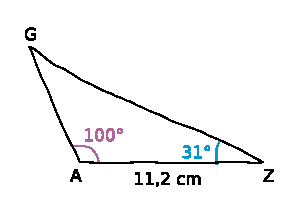
\includegraphics[width=3.3cm]{triangleGAZ} &  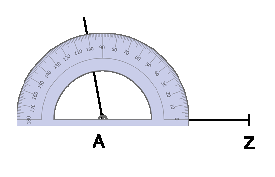
\includegraphics[width=3.0cm]{rapporteurAZ} & 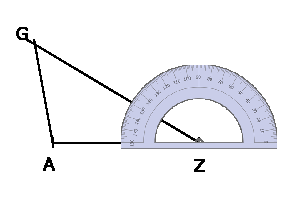
\includegraphics[width=3.0cm]{rapporteurGAZ} \\ 
 On effectue une figure à main levée en respectant la nature des angles (aigu ou obtus). & On trace un segment $[AZ]$ de longueur 11,2 cm. On construit un angle de sommet $A$, de côté $[AZ)$ et mesurant $100^\circ$. & On construit un angle de sommet $Z$, de côté $[ZA)$ et mesurant $31^\circ$. Les côtés des deux angles se coupent au point $G$. \\
\end{tabularx} \\

\end{exemple*1}

\exercice
Construis le triangle $SUD$ tel que :

$UD = 6$ cm ; $\widehat{SUD} = 65^\circ$ ; $\widehat{SDU} = 36^\circ$.
\vspace{4cm}
%\correction

\exercice
Construis le triangle $EST$ tel que :

$ET = 4,6$ cm ; $\widehat{SET} = 93^\circ$ et $\widehat{ETS} = 34^\circ$.
\vspace{2cm}
%\correction
 
\end{methode*1}

%%%%%%%%%%%%%%%%%%%%%%%%%%%%%%%%%%%%%%%%%%%%%%%%%%%%%%%%%%%%%%%%%%%%%%%%%%%%%%%%%
%\prof{
\begin{activite}[Manipulation: les droites remarquables dans le triangle]
\underline{Le but:} A l'aide de ficelles, construire d'abord un triangle quelconque puis placer les droites remarquables. Nommer le point d'intersection de ces droites.

\underline{Attention:} Prévoir un lieu suffisament grand pour que les élèves puissent travailler au sol, par groupe.\\

Constituer 4 groupes de travail.\\
\underline{Matériel(par groupe):}
\begin{itemize}
\item 1 grande corde "fermeé"
\item 3 petites cordes colorées
\end{itemize}
\underline{Matériel(pour la classe):}
\begin{itemize}
\item lots étiquettes droites remarquables et points d'intersection
\item un appareil photo
\item le matériel de géométrie pour tracer au tableau
\end{itemize}
\underline{déroulement (version 1: découverte):} Prévoir 2 périodes de cours.\\
Donner à chaque groupe une corde "triangle" et un lot de trois cordes  "droites".
\begin{itemize}
\item \underline{médiatrices:} Demander aux élèves de placer une corde de telle sorte qu'elle coupe un côté du triangle en son milieu, perpendiculairement. Faire les 3 médiatrices. Distribuer une étiquette "médiatrices" et "centre du cercle circonscrit" à chaque groupe. Faire une photo.
\item \underline{médianes:} Demander aux élèves de placer une corde qui passe par un sommet du triangle et qui coupe le côté opposé en son milieu. Faire les 3 médianes. Distribuer une étiquette "médianes" et "centre de gravité" à chaque groupe. Faire une photo.
\item \underline{hauteurs:} Demander aux élèves de placer une corde qui passe par un sommet et qui coupe le côté opposé perpendiculairement. Faire les 3 hauteur. Distribuer une étiquette "hauteurs" et "orthocentre" à chaque groupe. Faire une photo.
\item \underline{bissectrices:} Demander aux élèves de placer une corde qui coupe l'angle en deux parties égales. Faire les 3 hauteurs. Distribuer une étiquette "hauteurs" et "centre du cercle inscrit" à chaque groupe. Faire une photo.\\\\
Le travail du professeur est alors de construire un livret contenant une photo d'illustration de chacune des droites, la définition et un schéma réacapitulatif, personnalisé pour chaque groupe.
\end{itemize}
Attention: des explications complémentaires intermédiaires sont indispensables. Notamment préciser la nature de ces droite (demi-droite), en faisant bien attention que les cordes matérialisant les bissectrices partent du sommet de l'angle alors que les autre droites dépassent.
\underline{déroulement (version 2: bilan fin de séance):} Prévoir une période de cours.\\
Donner à chaque groupe une corde "triangle" et un lot de trois cordes  "droites".\\
Distribuer à chaque groupe une étiquette "droites".\\
Trois élèves doivent maintenir au sol les trois sommets du triangle. Les autres élèves du groupe, doivent alors placer le plus précisément possible, les trois droites remarquables indiquées sur leur étiquette.\\
Attention: il faut bien expliquer aux élèves "sommets" qu'ils ne doivent pas bouger sinon le triangle change et tout le travail est à recommencer.\\
Un fois que les trois droites sont matérialisées, les élèves appellent le professeur qui vérifie leur travail et les questionne sur le point d'intersection. On place en suite l'étiquette "p. d'intersection". On prend une photo souvenir!\\\\
Le travail du professeur est alors de construire un livret contenant une photo d'illustration de chacune des droites, la définition et un schéma réacapitulatif.


\end{activite}
%}



\newpage

%%%%%%%%%%%%%%%%%%%%%%%%%%%%%%%%%%%%%%%%%%%%%%%%%%%%%%%%%%%%%%%%%%%%%%%%%%%%%%%%%
%Médiatrice

 \begin{aconnaitre}
Les médiatrices des trois côtés d'un triangle sont \MotDefinition{concourantes}{}.

Leur point d'intersection est le centre du \MotDefinition{cercle circonscrit}{} au triangle. Ce cercle passe par les trois sommets du triangle.
\end{aconnaitre}

 \vspace{2em}
 
 \begin{methode*1}[Construire le cercle circonscrit à un triangle]
 
\begin{remarque}
Il suffit de tracer les médiatrices de deux côtés pour déterminer le centre du cercle circonscrit.
 \end{remarque}
 
 \begin{exemple*1}
Trace le cercle circonscrit au triangle $PAF$ :
 \begin{tabularx}{\textwidth}{X|X|X}
 
\includegraphics[width=3.2cm]{triangleFAP} &  
\includegraphics[width=3.2cm]{triangleFAOP} & 
\includegraphics[width=3.2cm]{triangle_cercleFAOP} \\ 
 On construit la médiatrice du segment $[AP]$. & On construit la médiatrice du segment $[FA]$. Soit $O$ le point d'intersection des deux médiatrices. & Le cercle circonscrit est le cercle de centre $O$ et de rayon $OA$ (ou $OF$ ou $OP$). \\
\end{tabularx} \\

\end{exemple*1}

\exercice
Construis le triangle $FEU$ tel que :

$FE = 6$ cm ; $EU = 3,7$ cm et $UF = 3,5$ cm. Trace le cercle circonscrit au triangle $FEU$.
\vspace{4cm}
%\correction

\exercice
Construis le triangle $EAU$ et son cercle circonscrit sachant que : $EA = 6,1$ cm ; $AU = 3$ cm et $UE = 4,9$ cm.

\vspace{2cm}
%\correction

\end{methode*1}



%%%%%%%%%%%%%%%%%%%%%%%%%%%%%%%%%%%%%%%%%%%%%%%%%%
%Médiane


\newpage

\begin{definition}
Dans un triangle, une \MotDefinition{médiane}{} est une droite qui passe par un sommet du triangle et par le milieu du côté opposé à ce sommet.

Les trois médianes d'un triangle sont concourantes en un point, noté G, et appelé \MotDefinition{centre de gravité}{} du triangle.
\end{definition}

\vspace{2em}

\begin{methode*1}[Construire le centre de gravité d'un triangle]

\begin{remarque}
Puisque les trois médianes sont concourantes, il suffit d'en tracer deux pour déterminer le centre de gravité.
 \end{remarque}

 \begin{exemple*1}
 Trace la centre de gravité du triangle $ABC$ :
 \begin{tabularx}{\textwidth}{X|X|X}
 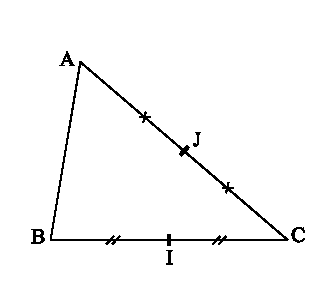
\includegraphics[width=3.2cm]{CentreGravite1} &  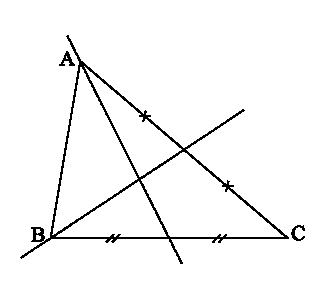
\includegraphics[width=3.2cm]{CentreGravite2} & 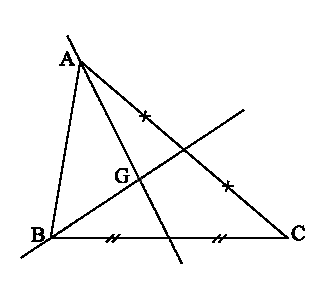
\includegraphics[width=3.1cm]{CentreGravite3} \\ 
 On trace le milieu de deux des côtés (ici I et J). & On trace les médianes passant par ces deux milieux & Le centre de gravité G est le point d'intertection des médianes. \\
\end{tabularx} \\

\end{exemple*1}

 
\exercice
Construis le triangle $CLE$ tel que 
$CL = 4,5$ cm ; $CE = 5,2$ cm et $\widehat{CLE} = 78^\circ$ puis trace son centre de gravité.
%\correction


\end{methode*1}


%%%%%%%%%%%%%%%%%%%%%%%%%%%%%%%%%%%%%%%%%%%%%%%%%%
%Hauteurs

\newpage

\begin{definition}
Dans un triangle, une \MotDefinition{hauteur}{} est une droite qui passe par un sommet du triangle et qui est perpendiculaire au côté opposé à ce sommet.

Les trois hauteurs d'un triangle sont concourantes en un point, noté H, et appelé \MotDefinition{orthocentre}{} du triangle.
\end{definition}

\vspace{2em}

\begin{methode*1}[Construire les hauteurs d'un triangle]

 \begin{exemple*1}
 Trace la hauteur relative au côté $[BR]$ :
 \begin{tabularx}{\textwidth}{X|X|X}
 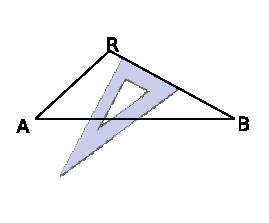
\includegraphics[width=3.2cm]{triangleARB_1} &  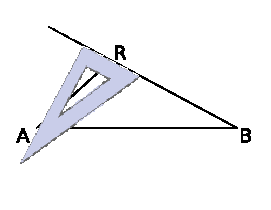
\includegraphics[width=3.2cm]{triangleARB_2} & 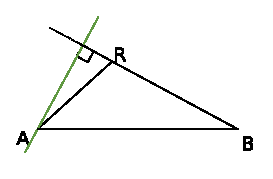
\includegraphics[width=3.1cm]{triangleARB_3} \\ 
 On positionne l'équerre perpendiculairement au côté $[BR]$. & On fait glisser l'équerre jusqu'au point $A$. Il faut parfois prolonger le côté $[BR]$. & La hauteur relative au côté $[BR]$ est la droite perpendiculaire au côté $[BR]$ et passant par $A$. \\
\end{tabularx} \\

\end{exemple*1}

\begin{remarque}
On dit aussi «hauteur issue du sommet $A$» pour nommer la hauteur relative au côté $[BR]$.
 \end{remarque}
 
\exercice
Construis le triangle $CAR$ tel que 
$CA = 4,6$ cm ; $AR = 4,3$ cm et $\widehat{CAR} = 102^\circ$ puis trace la hauteur issue de $R$ et celle issue de $C$.
\vspace{2cm}
%\correction
     
\exercice
Construis un triangle $TAX$ tel que 

$TA = 6,3$ cm ; $\widehat{TAX} = 57^\circ$ et $\widehat{ATX} = 63^\circ$ puis trace ses hauteurs.
\vspace{2cm}
%\correction

\exercice
Construis un triangle $BUS$ tel que :

$BU = 6,4$ cm ; $US = 4,8$ cm et $BS = 8$ cm. Trace les trois hauteurs de ce triangle.
%\correction

\end{methode*1}



%%%%%%%%%%%%%%%%%%%%%%%%%%%%%%%%%%%%%%%%%%%%%%%%%%
%Bissectrices

 \newpage
 
 \begin{aconnaitre}
Les trois bissectrices des angles d'un triangle sont concourantes. 

Leur point d'intersection est le \MotDefinition{centre du cercle inscrit}{} dans le triangle. Ce cercle est tangent aux trois côtés du triangle.
 \end{aconnaitre}
 
 \vspace{2em}
 
 \begin{methode*1}[Centre du cercle inscrit dans un triangle]
 
 \begin{remarque}
Il suffit de tracer les bissectrices de deux angles pour déterminer le centre du cercle inscrit.
 \end{remarque}
 
 \begin{exemple*1}
 Construis un triangle $MER$ et son cercle inscrit de centre $O$ :
 \begin{tabularx}{\textwidth}{X|X|X}
 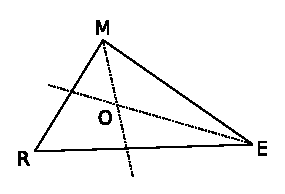
\includegraphics[width=3.2cm]{triangleMRE} &  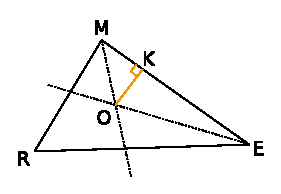
\includegraphics[width=3.2cm]{triangleMREK} & 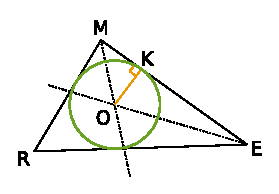
\includegraphics[width=3.2cm]{triangle_cercleMREK} \\ 
 On trace les bissectrices de deux des trois angles du triangle $MER$. Elles se coupent en $O$, le centre du cercle inscrit. & On trace la perpendiculaire à $(ME)$ passant par le point $O$. Elle coupe $[ME]$ en $K$. On obtient ainsi un rayon $[OK]$ du cercle inscrit dans le triangle $MER$. & On trace le cercle de centre $O$ passant par $K$. \\
 \end{tabularx} \\

\end{exemple*1}
 
 \exercice
Construis un triangle $RAS$ tel que 

$RA = 7$ cm ; $AS = 8$ cm et $RS = 9$ cm puis son cercle inscrit.
%\correction
 
 \end{methode*1}



\exercicesbase
\begin{colonne*exercice}

\serie{Autour du triangle}

\begin{exercice}
Complète les phrases en utilisant les mots « côté », « sommet », « triangle » et « opposé » : \\[-3em]
\begin{minipage}[c]{0.26\linewidth}
 \vspace{1.5cm}
 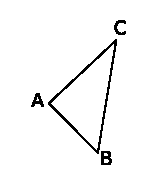
\includegraphics[width=1.8cm]{triangleCAB_vert}
 \end{minipage} \hfill%
 \begin{minipage}[t]{0.68\linewidth}
  \begin{enumerate}
   \item $ABC$ est un \dotfill
   \item $[AB]$ est un  \dotfill
   \item $B$ est un  \dotfill
   \item $[BC]$ est  \dotfill au sommet $A$ ;
   \item $B$ est le  \dotfill au  \dotfill $[AC]$ ;
   \end{enumerate}
 \end{minipage} \\
\end{exercice}


\begin{exercice}[Triangles particuliers]
 \begin{center} 
\includegraphics[width=2.5cm]{triangleGHI_rose} \qquad 
\includegraphics[width=2.4cm]{triangleEDF_brun} \end{center}
 Quelle est la nature du triangle $GHI$ ? Du triangle $DEF$ ? Justifie tes réponses.
\end{exercice}

\begin{exercice}[Reconnaître]
Donne, en justifiant, la nature de chacun des triangles s'il est particulier :
\begin{colenumerate}{4}
 \item 
 
 
\includegraphics[width=1.2cm]{reconnaitre1}
 \item 
 
 
\includegraphics[width=1.3cm]{reconnaitre2}
 \item 
 
 
\includegraphics[width=1.6cm]{reconnaitre3}
 \item 
 
 
\includegraphics[width=1.4cm]{reconnaitre4}
 \end{colenumerate}
\end{exercice}


\begin{exercice}[Avec le codage]
\begin{center} 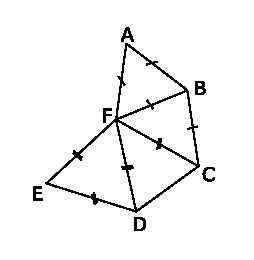
\includegraphics[width=3cm]{codage} \end{center}
\begin{enumerate}
 \item Quels sont les triangles équilatéraux ?
 \item Quels sont les triangles isocèles que l'on peut tracer en joignant des points de la figure ?
 \end{enumerate}
\end{exercice}


%%%%%%%%%%%%%%%%%%%%%%%%%%%%%%%%%%%%%%%%%%%%%%%%%%%%%%%%%%%%
\vspace{2em}
\serie{Constructions}

\begin{exercice}
Indique si chacun des triangles donnés ci-dessous est constructible ou non :

\includegraphics[width=2cm]{triangleMON} \hfill \includegraphics[width=2cm]{triangleWYX} \hfill \includegraphics[width=2cm]{triangleBCA}
\end{exercice}


\begin{exercice}
Explique pourquoi il est impossible de construire de tels triangles :

\hfill \includegraphics[width=5.7cm]{triangles_impos} \hfill 
\end{exercice}


\begin{exercice}
Construis les figures suivantes :

\hfill \includegraphics[width=6cm]{triangles_colores} \hfill 
\end{exercice}


\begin{exercice}
Dans chaque cas, effectue un croquis puis construis la figure.

 \begin{enumerate}
  \item Trace un triangle $FIN$ rectangle en $F$ tel que $FI = 5$ cm et $NF = 6$ cm ;
  \item Trace un triangle $TRS$ rectangle en $S$ tel que $TS = 72$ mm et $SR = 85$ mm ;
  \item Trace un triangle $GLU$ rectangle en $L$ tel que $LG = 8$ cm et $GU = 10$ cm.
  \end{enumerate}
\end{exercice}


\begin{exercice}[Construis \ldots]
 \begin{enumerate}
  \item Construis un triangle $MNO$ équilatéral de côté 5 cm ;
  \item Construis un triangle isocèle $STU$ isocèle en $S$ tel que $ST = 58$ mm et $TU = 32$ mm ;
  \item Construis un triangle $ABC$ tel que $AB = 6$ cm ; $BC = 5,2$ cm et $CA = 42$ mm.
  \end{enumerate}
\end{exercice}

%%%%%%%%%%%%%%%%%%%%Mise en page
\newpage
%%%%%%%%%%%%%%%%%%%%%%%%%%%%%%%%%%

\begin{exercice}
Quelle figure correspond au programme de construction suivant ? Justifie ta réponse.
 \begin{itemize}
  \item Construis un triangle $ABC$ rectangle en $A$ ;
  \item Construis $d_1$ la parallèle à $(BC)$ passant par $A$ ;
  \item Construis $d_2$ la médiatrice du segment $[AB]$ ;
  \item Place $D$ le point d'intersection des droites $d_1$ et $d_2$.
  \end{itemize}
  \begin{colenumerate}{2}
   \item \includegraphics[width=2.9cm]{triangleCABD_1}
   \item \includegraphics[width=1.9cm]{triangleCABD_2}   
   \item \includegraphics[width=2.5cm]{triangleCABD_3}
   \item \includegraphics[width=2.6cm]{triangleCABD_4}
   \end{colenumerate}
\end{exercice}


\begin{exercice}[Demandez le programme]
Remets les consignes du programme de construction dans l'ordre :
\begin{center} \includegraphics[width=4.1cm]{programme} \end{center}
 \begin{itemize}
  \item Trace la droite $d'$ parallèle à $(BC)$ passant par $A$ ;
  \item Nomme $O$ le point d'intersection de $d$ et $d'$ ;
  \item Trace un triangle $ABC$ rectangle en $A$, tel que $AB = 8$ cm et $AC = 6$ cm ;
  \item Trace la droite $d$ perpendiculaire à $d'$ et passant par $B$.
  \end{itemize}
\end{exercice}


\begin{exercice}[Triangle et losange]
 \begin{enumerate}
  \item Construis un triangle isocèle $ABC$ isocèle en $C$ tel que $AB = 3,5$ cm et $AC = 4,2$ cm ;
  \item Complète la figure avec la construction du point $D$ de sorte que $ACBD$ soit un losange ;
  \item Construis un triangle équilatéral $ABE$.
Qu'observes‑tu ?
   \end{enumerate}
\end{exercice}


\begin{exercice}
Trace un triangle $ABC$ isocèle en $A$ tel que $AB = 5$ cm et $BC = 3$ cm et un triangle $BCD$ isocèle en $D$ tel que $BD = 3,5$ cm.
\end{exercice}


\begin{exercice}[Le même triangle ?]
 \begin{enumerate}
  \item Trace un triangle $TRI$ tel que 
  
  $\widehat{TRI} = 45^\circ$ et  $\widehat{TIR} = 110^\circ$ ;
  \item Tes camarades obtiendront‑ils forcément un triangle identique au tien ?
  \end{enumerate}
\end{exercice}


\begin{exercice}
Dans chaque cas, effectue un croquis :
 \begin{enumerate}
  \item $SUR$ est un triangle tel que 
  
  $SU = 4,5$ cm, $\widehat{USR} = 60^\circ$ et $\widehat{RUS} = 40^\circ$ ;
  \item $QTD$ est un triangle tel que 
  
  $QT = 10$ cm, $TD = 7$ cm et $\widehat{QTD} = 70^\circ$ ;
  \item $MFV$ est un triangle tel que 
  
  $MF = 9$ cm, $FV = 12$ cm et $MV = 6$ cm.
  \end{enumerate}
\end{exercice}


\begin{exercice}[Reporter pour reproduire]
Reproduis les triangles suivants en utilisant uniquement une règle non graduée et un compas :
\begin{center} \includegraphics[width=7.1cm]{reproduire} \end{center}
\end{exercice}


\begin{exercice}
Après avoir effectué un croquis, construis les triangles suivants :
 \begin{enumerate}
  \item $GHI$ est un triangle tel que 
  
  $GH = 8$ cm, $HI = 5$ cm et $GI = 6$ cm ;
  \item $MNO$ est un triangle tel que 
  
  $MN = 4,5$ cm, $MO = 7$ cm et $\widehat{NMO} = 48^\circ$ ;
  \item $DEF$ est un triangle tel que 
  
  $DE = 8$ cm, $\widehat{FDE} = 45^\circ$ et $\widehat{FED} = 28^\circ$. 
  \end{enumerate}
\end{exercice}


%%%%%%%%%%%%%%%%%%%%Mise en page
\newpage
%%%%%%%%%%%%%%%%%%%%%%%%%%%%%%%%%%

\begin{exercice}
Dans chaque cas, effectue un croquis :
 \begin{enumerate}
  \item $POL$ est un triangle isocèle en $P$ tel que $PO = 14$ cm et $LO = 5$ cm ;
  \item $MER$ est un triangle équilatéral tel que $ME = 5$ cm ;
  \item $FAC$ est un triangle rectangle en $C$ tel que 
  
  $\widehat{AFC}= 50^\circ$ et $CA = 6,5$ cm.  
  \end{enumerate}
\end{exercice}


\begin{exercice}
Dans chaque cas, fais un croquis et construis :
 \begin{enumerate}
  \item $VUZ$ est un triangle isocèle en $U$ tel que 
  
  $VU = 6,5$ cm et $VZ = 4,5$ cm ;
  \item $KGB$ est un triangle équilatéral tel que 
  
  $KG = 6$ cm ;
  \item $CIA$ est un triangle rectangle en $C$ tel que $\widehat{CIA} = 37^\circ$ et $CI = 5,5$ cm ;
  \item $RTL$ est un triangle isocèle en $T$ tel que $RT = 8$ cm et $\widehat{TRL} = 48^\circ$.
  \end{enumerate}
\end{exercice}


\begin{exercice}
Sur ton cahier, reproduis en vraie grandeur la figure ci-dessous :
\begin{center} \includegraphics[width=6.9cm]{construction70} \end{center}
Écris ensuite le programme de construction.
\end{exercice}


\begin{exercice}
Dans chaque cas, fais un croquis et construis :
 \begin{enumerate}
  \item $EFG$ est un triangle tel que 
  
  $EF = 7,5$ cm, $\widehat{EFG} = 49^\circ$ et $\widehat{EGF} = 72^\circ$ ;
  \item $PLM$ est un triangle équilatéral de périmètre 15 cm ;
  \item Le triangle $RST$ est isocèle en $S$ de périmètre 13 cm et tel que $ST = 4$ cm ;
  \item Le triangle $AYB$ est isocèle et rectangle en $Y$ tel que $BA = 7$ cm ;
  \item Le triangle $OCI$ est isocèle en $I$ tel que $CO = 4,5$ cm et $\widehat{CIO} = 30^\circ$.
  \end{enumerate}
\end{exercice}


%%%%%%%%%%%%%%%%%%%%Mise en page
\vspace{3em}
%%%%%%%%%%%%%%%%%%%%%%%%%%%%%%%%%%

%%%%%%%%%%%%%%%%%%%%%%%%%%%%%%%%%%%%%%%%%%%%%%%%%%%%%%%%%%%%

\serie{Droites remarquables}

\begin{exercice}[Hauteurs d'un triangle]
Construis un triangle $BON$ tel que 

$BO = 68$ mm, $BN = 62$ mm et $NO = 45$ mm.

Trace :
\begin{itemize}
 \item En noir, la perpendiculaire à $(BN)$ passant par $O$ ;
 \item En rouge, la perpendiculaire à $(NO)$ passant par $B$ ;
 \item En vert, la perpendiculaire à $(BO)$ passant par $N$. Que remarques‑tu ?
 \end{itemize}
\end{exercice}


\begin{exercice}[Hauteur (« relative à » ou « issue de »)]
\begin{enumerate}
 \item Construis un triangle $AVE$ quelconque puis trace :
 \begin{itemize}
  \item En bleu, la hauteur issue du sommet $E$ ;
  \item En noir, la hauteur issue du sommet $A$ ;
  \item En rouge, la hauteur relative à $[AE]$.
  \end{itemize}
 \item Observe ces trois hauteurs. Quelle remarque peux-tu faire ?
 \end{enumerate}
\end{exercice}


\begin{exercice}[À l'intérieur ou pas ?]
\begin{enumerate}
 \item Construis un triangle $DER$ ayant tous ses angles aigus. Trace les hauteurs de ce triangle ;
 \item Construis un triangle $NRV$ tel que $\widehat{NRV}$ soit un angle obtus. Trace les hauteurs de ce triangle ;
 \item Construis un triangle $GHT$ rectangle en $T$. Trace les hauteurs de ce triangle ;
 \item Observe les trois figures. Quelles remarques peux-tu faire ?
 \end{enumerate}
\end{exercice}


\begin{exercice}[Médiatrices dans un triangle]
\begin{enumerate}
 \item Construis un triangle $ABC$ tel que $AB = 5,7$ cm, $AC = 5,3$ cm et $BC = 7$ cm.
 \item Construis les médiatrices des segments $[AB]$ et $[CB]$. Note $O$ leur point d'intersection.
 \item Construis la médiatrice du segment $[AC]$. Que constates‑tu ?
 \item Trace le cercle de centre $O$ passant par $A$. Comment s'appelle ce cercle ?
 \end{enumerate}
\end{exercice}

%%%%%%%%%%%%%%%%%%%%Mise en page
\newpage
%%%%%%%%%%%%%%%%%%%%%%%%%%%%%%%%%%


\begin{exercice}[Bissectrice dans un triangle]
\begin{enumerate}
 \item Trace un triangle $UST$ tel que 
 
 $UT = 3$ cm ; $US = 5$ cm et $ST = 7$ cm ;
 \item Construis les bissectrices des angles $\widehat{UST}$, $\widehat{UTS}$ et $\widehat{TUS}$.
 \end{enumerate}
 \vspace{-0.3cm}
Que constates‑tu ?
\end{exercice}


\begin{exercice}[Croquis et codages]
\begin{enumerate}
 \item Construis le triangle $TOC$ tel que 
 
 $TO = 8$ cm, $OC = 4,5$ cm et $CT = 6$ cm ;
 \item Trace puis code :
  \begin{itemize}
   \item En rouge, la hauteur issue de $O$ ;
   \item En bleu, la médiatrice de $[TO]$ ;
   \item En noir, la médiane relative à $[OC]$.
   \end{itemize} 
 \end{enumerate}
\end{exercice}

\begin{exercice}
Pour chaque triangle, indique si la droite (d) est une médiatrice, une hauteur ou une bissectrice.
 \begin{colenumerate}{2}
 \item

 \includegraphics[height=1.5cm]{DroiteRemarquable_1}

 \dotfill
 \item
 
 \includegraphics[height=1.5cm]{DroiteRemarquable_2}

 \dotfill
 \item
 
 \includegraphics[height=1.5cm]{DroiteRemarquable_3}

 \dotfill
 \item
 
 \includegraphics[height=1.5cm]{DroiteRemarquable_4}

 \dotfill

 \end{colenumerate}

\end{exercice}


%%%%%%%%%%%%%%%%%%%%Mise en page
\vspace{3cm}
%%%%%%%%%%%%%%%%%%%%%%%%%%%%%%%%%%


\begin{exercice}
Pour chaque triangle, indique si la droite $d$ est une médiatrice, une hauteur, une bissectrice ou une médiane.
\begin{colenumerate}{3}
 \item
 
 \includegraphics[width=2.3cm]{cas_1}

 \dotfill
 \item
 
 \includegraphics[width=1.6cm]{cas_2}

 \dotfill
 \item
 
 \includegraphics[width=1.7cm]{cas_3}

 \dotfill
 \item
 
 \includegraphics[width=1.6cm]{cas_4}

 \dotfill
 \item
 
 \includegraphics[width=1.8cm]{cas_5}

 \dotfill
 \item
 
 \includegraphics[width=1.8cm]{cas_6}

 \dotfill
 \end{colenumerate}
\end{exercice}


\begin{exercice}
Complète.
\begin{center}
 \includegraphics[width=0.3\textwidth]{DroiteRemarquable_6}
\end{center}
\begin{itemize}
\item $(d_1)$ est \dotfill
\item $(d_2)$ est \dotfill
\item $(d_3)$ est \dotfill
\end{itemize}
\end{exercice}


\begin{exercice}
Observe le triangle ABC et complète les phrases suivantes sachant que I et J sont les milieux respectifs des côtés [AB] et [BC].
\begin{center}
 \includegraphics[width=0.3\textwidth]{DroiteRemarquable_5}
\end{center}

\begin{itemize}
\item \dots \dots \hspace{1em} est la bissectrice de $\widehat{ABC}$.
\item \dots \dots \hspace{1em} est la médiatrice du segment [AB].
\item \dots \dots \hspace{1em} est la hauteur relative à [AB].
\item \dots \dots \hspace{1em} est la médiatrice du segment [BC].
\end{itemize}


\end{exercice}



\begin{exercice}[Vocabulaire] \label{triangles_vocabulaire}
\begin{enumerate}
 \item Construis un triangle $BOA$ tel que $BO = 5$ cm, $OA = 7$ cm et $AB = 8$ cm. Trace la droite $d_1$ perpendiculaire à $[BO]$ et passant par $A$ ;
 \item Trace la droite $d_2$ perpendiculaire au segment $[OA]$ et passant par son milieu ;
 \item Trace la droite $d_3$ qui coupe l'angle $\widehat{OBA}$ en deux angles égaux ;
 \item Trace la droite $d_4$ qui passe par $O$ et par le milieu de $[BA]$ ;
 \item Détermine quelle(s) droite(s) représente(nt) une hauteur du triangle ;
 \item Détermine quelle(s) droite(s) représente(nt) une médiatrice ;
 \item Détermine quelle(s) droite(s) représente(nt) une bissectrice ;
 \item Détermine quelle(s) droite(s) représente(nt) une médiane.
 \end{enumerate}
\end{exercice}


\begin{exercice}[Médiane]
\begin{enumerate}
 \item Construis le triangle $BOA$ identique à l'exercice \ref{triangles_vocabulaire} :
 \begin{itemize}
  \item la médiane issue de $O$ ;
  \item la médiane relative au côté $[AO]$ ;
  \item la médiane issue de $A$.
  \end{itemize}
 \item Observe la figure. Que peux-tu dire de ces trois médianes ?
 \end{enumerate}
\end{exercice}


\begin{exercice}[Hauteurs]
Trace les hauteurs des triangles suivants.

\vspace{2em}
\begin{center}
 \includegraphics[width=0.3\textwidth]{Hauteurs_1}
 
\vspace{1em}

 \includegraphics[width=0.3\textwidth]{Hauteurs_2}
\end{center}
\vspace{1em}
\end{exercice}


\begin{exercice}[Cercle circonscrit]
Trace le cercle circonscrit des triangles suivants.

\vspace{2em}
\begin{center}
 \includegraphics[width=0.3\textwidth]{CercleCirconscrit_1}

\vspace{5em}
 \includegraphics[width=0.3\textwidth]{CercleCirconscrit_2}
\end{center}
\vspace{2em}
\end{exercice}



\begin{exercice}[Cercle inscrit]
Dans chaque cas, construis le triangle $ABC$ puis son cercle inscrit :
\begin{enumerate}
 \item $AC = 8$ cm, $\widehat{BAC} = 60^\circ$ et $\widehat{ACB} = 50^\circ$ ;
 \item $AC = 10$ cm, $AB = 8$ cm et $\widehat{BAC} = 45^\circ$ ;
 \item $ABC$ est isocèle en $A$ tel que $AB = 9$ cm et $BC = 6$ cm ;
 \item $ABC$ est un triangle équilatéral de côté 7,5 cm.
 \end{enumerate}
\end{exercice}


\begin{exercice}
Trace un triangle dont le cercle inscrit a un rayon de 2,7 cm.
\end{exercice}


%%%%%%%%%%%%%%%%%%%%Mise en page
\newpage
%%%%%%%%%%%%%%%%%%%%%%%%%%%%%%%%%%

\begin{exercice}[Des triangles, beaucoup de triangles]
\begin{enumerate}
 \item Parmi les onze triangles tracés, indique ceux qui sont isocèles, rectangles ou équilatéraux.
 \begin{center} \includegraphics[width=8.3cm]{triangles_many} \end{center}
 \item Construis les triangles suivants : $AGJ$, $AHB$ et $CED$. Que constates-tu ?
 \end{enumerate}
\end{exercice}

\end{colonne*exercice}


\exercicesappr
\begin{colonne*exercice}
\begin{exercice}[Plusieurs triangles]
\begin{itemize}
 \item $RAT$ est un triangle tel que $RA = 7$ cm ; $TA = 6$ cm et $\widehat{RAT} = 40^\circ$ ;
 \item $RIT$ est un triangle tel que $\widehat{RTI} = 57^\circ$ ; $\widehat{TRI} = 82^\circ$.
 \end{itemize}
\vspace{-0.5cm}
Dans chaque cas fais un croquis des triangles puis construis-les. Que remarques-tu ? 
\end{exercice}


\begin{exercice}[Triangles et cercle]
Construis un triangle $LAC$ isocèle en $C$ tel que $LA = 3$ cm et $LC = 5$ cm :
\begin{enumerate}
 \item Trace le cercle de centre $C$ passant par $A$. Que constates‑tu ?
 \item Construis si possible un triangle $ABC$ équilatéral tel que $B$ appartienne à ce cercle.
 \end{enumerate}
\end{exercice}


\begin{exercice}[À partir d'un programme]
Réalise la figure correspondant au programme de construction ci‑dessous :
\begin{itemize}
 \item Trace un triangle $ABC$ rectangle en $B$ avec $AB = 4$ cm et $BC = 6$ cm ;
 \item Trace le rectangle $ACDE$ avec $AE = 5$ cm de telle sorte que $B$ soit un point extérieur à $ACDE$ ;
 \item Trace la droite $d$ perpendiculaire à $(AB)$ passant par $A$ ;
 \item Trace $d'$ la médiatrice de $[DE]$ ;
 \item Place $F$ le point d'intersection de $d$ et $d'$ ;
 \item Trace la droite $d''$ parallèle à $(AC)$ passant par $B$.
 \end{itemize}
Que peux‑tu dire des droites $d'$ et $d''$ ? (Justifie)
\end{exercice}


\begin{exercice}[Avec des médiatrices]
Construis le triangle $ABC$ tel que $AB = 8$ cm ; $AC = 4$ cm et $BC = 6$ cm. Trace $d_1$ la médiatrice de $[AB]$ et $d_2$ la médiatrice de $[BC]$. Les droites $d_1$ et $d_2$ sont sécantes en $O$. Trace $d_3$ la parallèle à $(BC)$ passant par $O$. Que peux‑tu dire des droites $d_2$ et $d_3$ ?
\end{exercice}


\begin{exercice}[Avec le périmètre et les angles]
On veut tracer un triangle tel que son périmètre mesure 16 cm et deux de ses angles mesurent $64^\circ$ et $46^\circ$ :
\begin{enumerate}
 \item Effectue un croquis de ce triangle et calcule la mesure de son troisième angle ;
 \item Trace un segment $[DE]$ mesurant 16 cm et place $A$ tel que : $\widehat{ADE} = 32^\circ$ et $\widehat{AED} = 23^\circ$ (on a pris les moitiés de $64^\circ$ et $46^\circ$) ;
 \item Place un point $B$ sur le segment $[DE]$ à égale distance de $A$ et de $D$ puis un point $C$ sur le segment $[DE]$ à égale distance de $A$ et de $E$. Indique la nature des triangles $ABD$ et $ACE$ ;
 \item Mesure les angles des triangles $ABD$ et $ACE$ ;
 \item Compare le périmètre et les angles du triangle $ABC$ avec ceux du triangle cherché ;
 \item Trace un triangle $RST$ de périmètre 20 cm tel que $\widehat{RST} = 36^\circ$ et $\widehat{STR} = 68^\circ$.
 \end{enumerate}
\end{exercice}


\begin{exercice}[Un joli cercle d'amis]
\begin{enumerate}
 \item Kévin et Nicolas ont tous les deux leur arbre fétiche sous lequel ils aiment se reposer. Mais ils aiment aussi faire la course en partant chacun de leur arbre. Pour que la course soit équitable, il faut que l'arrivée soit située à la même distance des deux arbres.
 \begin{itemize}
  \item Sur ton cahier, place deux points $K$ et $N$ (distant de 4 cm) pour représenter les arbres de Kévin et de Nicolas. Construis ensuite un point à égale distance des deux arbres $K$ et $N$ et places-y un drapeau.
  \item Où placer l'arrivée pour que la course soit la plus courte possible ?
  \item Si Kévin et Nicolas veulent une course plus longue, où peuvent-ils encore planter le drapeau ? Quel est l'ensemble des points possibles pour l'arrivée ? Trace-le en bleu. 
  \end{itemize}
 \item Gabin a aussi son arbre et il aimerait bien jouer avec Nicolas au même jeu. Sur ton cahier, place un point $G$, comme sur la figure ci-dessous représentant l'arbre de Gabin.
 \begin{center} \includegraphics[width=4cm]{pointsKNG} \end{center}
 \begin{itemize}
  \item Trace \textbf{\textcolor{B2}{en rouge}} l'ensemble des points équidistants des arbres de Gabin et de Nicolas.
  \item Mais Kévin, désormais, s'ennuie. Il propose : « Organisons une course à trois ! ». Où peuvent-ils planter le drapeau ? Pourquoi ? 
  \item Yann n'a pas d'arbre à lui mais veut aussi courir. Nicolas dit : « Si tu veux jouer, ton arbre doit être aussi loin du drapeau que les nôtres ! » Place plusieurs points où pourrait être l'arbre de Yann. Où semblent se situer ces points ? 
  \item Trace l'ensemble des points où pourrait être l'arbre de Yann.
  \end{itemize}
 \end{enumerate}
\end{exercice}

\end{colonne*exercice}

\connaissances


\QCMautoevaluation{Pour chaque question, plusieurs réponses sont
  proposées.  Déterminer celles qui sont correctes.} 
  
\begin{QCM}
  \begin{GroupeQCM} 
    \begin{exercice}
      Si $CA = CB$ alors \ldots
      \begin{ChoixQCM}{4}
      \item $C$ est le milieu de $[AB]$
      \item le triangle $ABC$ est isocèle en $A$
      \item $A$ et $B$ sont sur un cercle de centre $C$
      \item le triangle $ABC$ est isocèle en $C$
      \end{ChoixQCM}
\begin{corrige}
     \reponseQCM{cd} 
   \end{corrige}
    \end{exercice}
    

    \begin{exercice}
      Un triangle $ABC$ est isocèle en $B$ alors \ldots
      \begin{ChoixQCM}{4}
      \item $AC = BC$
      \item $AB = BC$
      \item Le plus grand angle est $\widehat{ABC}$
      \item $\widehat{CAB} = \widehat{BCA}$
      \end{ChoixQCM}
\begin{corrige}
     \reponseQCM{bd}
   \end{corrige}
    \end{exercice}


    \begin{exercice}
      Si $RST$ est un triangle rectangle en $T$ alors \ldots
      \begin{ChoixQCM}{4}
      \item $RS = ST$
      \item $(ST) \perp (RS)$
      \item $(ST) \perp (TR)$
      \item $RS \geqslant ST$ et $RS \geqslant RT$
      \end{ChoixQCM}
\begin{corrige}
     \reponseQCM{cd}
   \end{corrige}
    \end{exercice}
    

    \begin{exercice}
      Sur la figure ci‑dessous, \ldots
      
     \begin{minipage}[c]{0.32\textwidth}
     \quad \includegraphics[width=3.5cm]{triangleACIB}
     \end{minipage} \hfill%
     \begin{minipage}[c]{0.66\textwidth}
     $d_1$ correspond à la droite $(CI)$
     
     $AI = IB$ et $CJ = BJ$
     \end{minipage} \\
      
      \begin{ChoixQCM}{4}
      \item la droite $d_1$ est la médiatrice du segment $[AB]$
      \item la droite $d_2$ est la médiatrice du segment $[CB]$
      \item le triangle $BCI$ est un triangle rectangle
      \item $d_3 \parallel (CB)$
      \end{ChoixQCM}
\begin{corrige}
     \reponseQCM{b}
   \end{corrige}
    \end{exercice}
    

\end{GroupeQCM}
\end{QCM}

  


\TravauxPratiques % pour nous "travailler en groupe"

\begin{TP}[Droite d'Euler]

\begin{enumerate}
\item Construis un triangle $DOC$ tel que $DO = 16$ cm, $OC = 12$ cm et $CD = 10$ cm.
\item Construis les hauteurs du triangle $DOC$ issues des sommets $D$, $O$ et $C$. Ces hauteurs sont concourantes. Nomme ce point d'intersection $H$ (ce point est l'orthocentre du triangle).
\item Trouve le centre $I$ du cercle circonscrit du triangle $DOC$.
\item Construis les trois médianes du triangle $DOC$. Ces médianes sont concourantes. Nomme ce point d'intersection $G$ (ce point est le centre de gravité du triangle).
\item Vérifie que les points $H$, $I$, $G$ sont alignés.

La droite qui passe par ces trois points est appelée la droite d'Euler. C'est le mathématicien Suisse Leonhard Euler (1707 - 1783) qui démontra en premier que ces points étaient alignés.
\end{enumerate}

\end{TP}

%%%%%%%%%%%%%%%%%%%%%%%%%%%%%%%%%%%%%%%%%%%%%%%%%%%%%%%%%%%%%%%%%%%%

\begin{TP}[Pavage par triangles curvilignes]

\partie{Un triangle curviligne}

\begin{enumerate}
 \item Réalisez la figure ci-dessous sachant qu'elle est composée d'un triangle équilatéral de 6 cm de côté et que le diamètre des disques est deux fois plus petits que la longueur d'un côté du triangle.
 \end{enumerate}
 
 \begin{center} \includegraphics[width=3.5cm]{t_curviligne} \end{center}

\partie{Pavage du plan}

\begin{enumerate}
 \item Sur une feuille A4, réalise le maximum de triangles curvilignes en les plaçant les uns contre les autres. Coloriez les figures selon votre inspiration.
 \item En plaçant les triangles curvilignes les uns contre les autres, réalisez des frises décoratives et comparez vos résultats avec les autres réalisations.
 
 \begin{center} \includegraphics[width=3.5cm]{pavage} \end{center}

 \end{enumerate}

\end{TP}



\recreation
\begin{enigme}[Belle figure]

Construis une figure analogue à partir d'un triangle $ABC$ isocèle de sommet principal $A$ tel que $BC = 10$ cm et $AC = 14$ cm :

\begin{center} \includegraphics[width=3.2cm]{t_artistique} \end{center}

 \end{enigme}
 
 
%%%%%%%%%%%%%%%%%%%%%%%%%%%%%%%%%%%%%%%%%%%%%%%%%%%%%%%%%%%%%

\begin{enigme}[Artistes en géométrie]

\begin{enumerate}
 \item Recherche des informations sur le peintre Pietr Mondrian et notamment sur ses œuvres peintes à Paris.
 \item Quelles figures géométriques sont souvent visibles dans ses toiles ?
 \item À la manière de Mondrian, sur une feuille blanche, trace un cadre avec, à l'intérieur, des droites parallèles verticales et horizontales. Puis colorie en t'inspirant des œuvres de cet artiste.
 \item L'artiste Vassily Kandinsky a aussi travaillé à partir de figures géométriques. Cite le nom de certaines de ses œuvres.
 \item Recherche d'autres artistes ayant travaillé avec des figures géométriques.
 \end{enumerate}
 
 \end{enigme}





